\documentclass[aspectratio=169,11pt]{beamer}

\usepackage[T1]{fontenc}
\usepackage{lmodern}
\usepackage{xcolor}
\usepackage{tikz}
\usetikzlibrary{positioning, arrows.meta, shapes.geometric, fit}
\usepackage{booktabs}
\usepackage{array}
\usepackage{listings}
\usepackage{textcomp}

\definecolor{navy}{HTML}{0A2540}
\definecolor{orange}{HTML}{D97706}
\definecolor{green}{HTML}{15803D}
\definecolor{grey}{HTML}{6B7280}
\definecolor{lightgrey}{HTML}{E5E7EB}
\definecolor{red}{HTML}{B91C1C}
\definecolor{codebg}{HTML}{F8FAFC}
\definecolor{lightorange}{HTML}{FED7AA}
\definecolor{lightnavy}{HTML}{DBEAFE}

\usecolortheme[named=navy]{structure}
\setbeamertemplate{navigation symbols}{}
\setbeamercolor{frametitle}{fg=navy}
\setbeamerfont{frametitle}{series=\bfseries,size=\Large}
\setbeamertemplate{footline}{%
  \hbox{\hspace{0.9em}\color{grey}\tiny exp27 \textperiodcentered\
    iter\_R4\_grow\_on\_sampled\_uniform\_M5 \textperiodcentered\ MarinFold 1B\hfill\insertframenumber{} / \inserttotalframenumber\hspace{0.9em}}\vspace{0.3em}}
\setbeamertemplate{frametitle}{%
  \vspace*{0.4em}\hspace*{0.6em}\insertframetitle\par
  \vspace*{-0.2em}\hspace*{0.6em}\textcolor{orange}{\rule{0.93\paperwidth}{1.2pt}}\vspace*{-0.4em}
}

\lstdefinestyle{code}{
  basicstyle=\ttfamily\small\color{navy},
  backgroundcolor=\color{codebg},
  frame=single, framerule=0.4pt, rulecolor=\color{navy},
  numbers=none, breaklines=false, showstringspaces=false,
  xleftmargin=0.6em, xrightmargin=0.6em,
  aboveskip=0.4em, belowskip=0.4em,
}
\lstdefinestyle{codesmall}{
  basicstyle=\ttfamily\scriptsize\color{navy},
  backgroundcolor=\color{codebg},
  frame=single, framerule=0.4pt, rulecolor=\color{navy},
  numbers=none, breaklines=false, showstringspaces=false,
  xleftmargin=0.6em, xrightmargin=0.6em,
  aboveskip=0.4em, belowskip=0.4em,
}

\newcommand{\code}[1]{\texttt{\small\color{navy}#1}}
\newcommand{\codeS}[1]{\texttt{\scriptsize\color{navy}#1}}

\begin{document}

% --- Slide 1: title ---
\begin{frame}[plain]
  \begin{center}
    \vspace{0.6cm}
    {\Huge\bfseries\color{navy}Sampled-prior + iterative seeding}\\[0.4cm]
    {\Large\color{navy}\ttfamily iter\_R4\_grow\_on\_sampled\_uniform\_M5}\\[0.7cm]
    {\large\color{green}\bfseries Mean LDDT 0.250 \textrightarrow{} 0.356 \quad (+42.8\%)}\\[0.3cm]
    {\large\color{navy}on the FoldBench-10 train set with MarinFold 1B}\\[1.2cm]
    {\small\color{navy}Two ideas, one pipeline:\\[0.3em]
     (1) sample contacts honestly with grammar-constrained decoding\\
     (2) iterate the model's own confident contact picks with a growing budget}\\[0.7cm]
    {\small\color{grey}\ttfamily Issue \#27 \textperiodcentered\ exp27}
  \end{center}
\end{frame}

% --- Slide 2: recap baseline ---
\begin{frame}[fragile]{Recap: the problem and the bars}
  MarinFold 1B is a Llama-arch LLM. The naive baseline reads
  distogram bins with zero context:
  \begin{lstlisting}[style=code]
prompt = <begin_sequence> <AAs> <begin_statements>
for (i, j) in all pairs:
    tail = <distance> <p_i> <p_j> <atom_i> <atom_j>
    distance_dist[i, j] = softmax(model(prompt + tail))[<d_*>]
  \end{lstlisting}
  \vspace{0.3em}
  \begin{itemize}
    \setlength\itemsep{0.3em}
    \item Baseline mean LDDT on 10 train proteins: \textbf{0.2496}.
    \item Original target (issue): mean LDDT $\geq 0.2746$ (\textbf{+10\%}). Cleared
          early by sharpening + naive seeding.
    \item Raised target (mid-experiment): mean LDDT $\geq 0.3744$
          (\textbf{+50\%}). The hard one.
    \item Wall-clock budget: $\leq 5\times$ baseline ($\leq 6920$\,s on one A100).
    \item GT-oracle (cheating, diagnostic only): 0.7167 — the model
          IS capable; bottleneck is honest contact prediction.
  \end{itemize}
\end{frame}

% --- Slide 3: previous best ---
\begin{frame}{Recap: previous best was pure iteration}
  \begin{columns}[T]
    \begin{column}{0.55\textwidth}
      \textbf{\ttfamily iter\_R4\_grow\_05\_10\_15\_25}\\[0.4em]
      For each of 4 rounds with a growing K:
      \begin{enumerate}
        \setlength\itemsep{0.15em}
        \item Pick top-$K$ contacts from the previous round's distogram
              (sum of bins $\leq 8$\,\r{A}; minimum prob 0.1; ordered
              long $>$ medium $>$ short).
        \item Build prefix:\\
              \codeS{<begin\_statements><$\{$range$\}$-range-contact><p\_i><p\_j>\ldots}
        \item Re-read distances at LDDT-shell pairs.
      \end{enumerate}
      \vspace{0.5em}
      $K$ per round: $0.5L, 1.0L, 1.5L, 2.5L$.
      \vspace{0.5em}\\
      \textbf{Result: mean LDDT 0.3511 (+40.7\%).}\\
      Chain wall: 4373\,s (3.16$\times$ baseline).\\[0.2em]
      4 / 10 proteins individually pass the +50\% bar.\\
      Still 0.023 short of the mean bar.
    \end{column}
    \begin{column}{0.43\textwidth}
      \begin{center}
        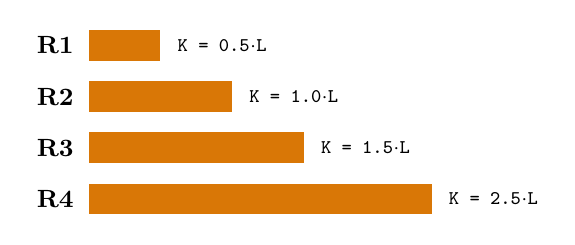
\begin{tikzpicture}[scale=0.65]
          \foreach[count=\i from 1] \rr/\kk/\ww in
              {1/0.5/1.4, 2/1.0/2.8, 3/1.5/4.2, 4/2.5/6.7} {
            \node[anchor=east, font=\small] at (-0.1, -\i + 0.35) {\textbf{R\rr}};
            \fill[orange] (0, -\i + 0.05) rectangle ++(\ww, 0.6);
            \node[anchor=west, font=\ttfamily\scriptsize] at (\ww + 0.15, -\i + 0.35)
              {K = \kk$\cdot$L};
          }
        \end{tikzpicture}
      \end{center}
      \vspace{0.6em}
      {\footnotesize\color{grey}\itshape Per-round contact budget.
        Round 1 picks from the \emph{naive baseline} distogram.}
    \end{column}
  \end{columns}
\end{frame}

% --- Slide 4: insight ---
\begin{frame}{Why add sampling? Different contacts}
  Pure iteration picks contacts by the model's
  \textbf{marginal} contact probability — for each pair $(i,j)$
  independently, sum $\Pr[d_{ij} < 8\,$\r{A}$]$. Pairs the model
  predicts confidently as contacts.\\[0.4em]
  But the model is autoregressive. \textbf{Joint} samples from
  \codeS{<begin\_statements> [...]} encode CO-occurring contacts —
  hints the model wouldn't reveal in marginal reads.\\[0.4em]
  \begin{center}
    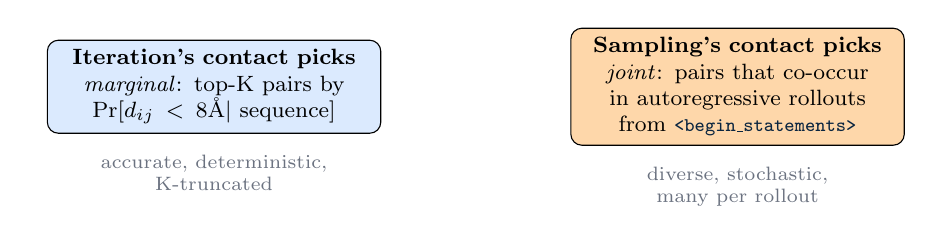
\begin{tikzpicture}[node distance=0.5cm and 1.0cm]
      \node[draw, rounded corners, fill=lightnavy, font=\footnotesize, align=center,
            text width=4.0cm] (marg) {%
        \textbf{Iteration's contact picks}\\
        \emph{marginal}: top-K pairs by\\
        $\Pr[d_{ij} < 8 $\r{A}$ \mid$ sequence$]$
      };
      \node[right=2.4cm of marg, draw, rounded corners, fill=lightorange,
            font=\footnotesize, align=center, text width=4.0cm] (joint) {%
        \textbf{Sampling's contact picks}\\
        \emph{joint}: pairs that co-occur\\
        in autoregressive rollouts\\
        from \codeS{<begin\_statements>}
      };
      \node[below=0.15cm of marg, font=\scriptsize\color{grey}, text width=4.5cm,
            align=center]
        {accurate, deterministic,\\ K-truncated};
      \node[below=0.15cm of joint, font=\scriptsize\color{grey}, text width=4.5cm,
            align=center]
        {diverse, stochastic,\\ many per rollout};
    \end{tikzpicture}
  \end{center}
  \vspace{0.4em}
  \textbf{They are complementary} — joint samples help where the marginal is weak,
  and iteration sharpens what the union proposes.
\end{frame}

% --- Slide 5: the sampling bug ---
\begin{frame}[fragile]{Sampling, attempt 1: the wrong cutoff}
  Natural autoregressive generation from \codeS{<begin\_statements>}
  emits \emph{any} statement next. Training docs interleave contacts
  and distances — \codeS{<distance>} is not a "boundary" token.
  \begin{lstlisting}[style=codesmall]
# WRONG: stop at first <distance>
sampling = SamplingParams(temperature=0.7, top_p=0.9, max_tokens=600,
                          stop=["<distance>", "<end>"])
out = llm.generate(prompt, sampling)
# -> emits 2 to 33 contact statements, then a <distance>, stop.
  \end{lstlisting}
  Per-protein contacts harvested per rollout:
  \begin{center}\small
    \begin{tabular}{lrrr}
      \toprule
      protein & 8eb9 (L=95) & 7y5j (L=102) & 7uk8 (L=394)\\
      \midrule
      naive sampling, stop-on-<distance> & 2 & 8 & 33 \\
      \textbf{(what we actually want)} & \textbf{100s} & \textbf{100s} & \textbf{100s} \\
      \bottomrule
    \end{tabular}
  \end{center}
  Result (M=1 average): mean LDDT \textbf{0.2568} (+2.9\%). Seed set too small.
\end{frame}

% --- Slide 6: the LP fix ---
\begin{frame}[fragile]{Sampling, attempt 2: contacts-only LP}
  Constrain the sampler with a custom \codeS{logits\_processor} that
  enforces the grammar of one contact statement, on repeat:\\[0.4em]
  \begin{center}
    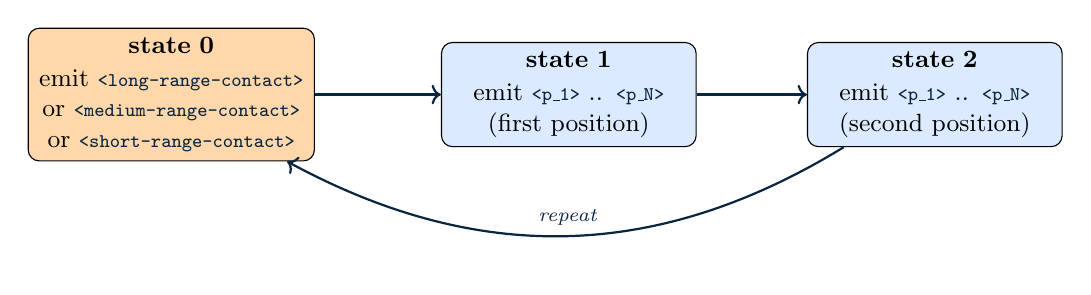
\begin{tikzpicture}[node distance=1.5cm and 1.1cm,
                        every node/.style={font=\small}]
      \node[draw, rounded corners, fill=lightorange, minimum width=3.4cm,
            text width=3.4cm, align=center] (s0)
        {\textbf{state 0}\\[0.1em]
         emit \codeS{<long-range-contact>}\\
         or \codeS{<medium-range-contact>}\\
         or \codeS{<short-range-contact>}};
      \node[right=1.6cm of s0, draw, rounded corners, fill=lightnavy,
            minimum width=3.0cm, text width=3.0cm, align=center] (s1)
        {\textbf{state 1}\\[0.1em]
         emit \codeS{<p\_1>} .. \codeS{<p\_N>}\\
         (first position)};
      \node[right=1.4cm of s1, draw, rounded corners, fill=lightnavy,
            minimum width=3.0cm, text width=3.0cm, align=center] (s2)
        {\textbf{state 2}\\[0.1em]
         emit \codeS{<p\_1>} .. \codeS{<p\_N>}\\
         (second position)};
      \draw[->, thick, navy] (s0) -- (s1);
      \draw[->, thick, navy] (s1) -- (s2);
      \draw[->, thick, navy] (s2) edge[bend left=30] node[above, font=\scriptsize\itshape]
        {repeat} (s0);
    \end{tikzpicture}
  \end{center}
  \vspace{0.3em}
  LP receives generated tokens; \codeS{state = len(gen) \% 3}. All other
  tokens get $-\infty$ logits. The whole \codeS{max\_tokens=900} budget
  is spent emitting contact statements: \textbf{225 to 300 unique (i,j)
  pairs per rollout}.
\end{frame}

% --- Slide 7: range-token surprise ---
\begin{frame}{Surprise: the model's range-token prior is broken}
  With the LP allowing all 3 range tokens, sample at $T=0.7$:
  \vspace{0.3em}
  \begin{center}
    \begin{tabular}{lrrr}
      \toprule
      protein (L) & long & medium & short \\
      \midrule
      8eb9 (95)   & 3   & 222 & 0 \\
      8baq (208)  & 1   & 295 & 0 \\
      7uk8 (394)  & 1   & 295 & 0 \\
      \bottomrule
    \end{tabular}
  \end{center}
  \vspace{0.5em}
  \textbf{$\sim 99\%$ medium-range across every protein.}\\
  The model treats \codeS{<medium-range-contact>} as the overwhelmingly likely
  next-statement token.\\[0.5em]
  But the medium-range pairs aren't necessarily the most informative for LDDT —
  long-range contacts pin down the global fold, short-range ones lock in local
  topology. Sampling at the model's natural prior gives 296 medium-range pairs
  and basically no signal about the rest.\\[0.4em]
  \textbf{M=1 result with model prior: 0.2219 (\textcolor{red}{$-11.1\%$}) — WORSE than baseline.}
  \quad{\small\itshape (\codeS{range\_strategy=model})}
\end{frame}

% --- Slide 8: entropy probe ---
\begin{frame}{Is it the prior or the knowledge? (entropy probe)}
  For each range token $r$, ask: \emph{after we emit $r$, how
  informative is the model's distribution over the next position?}\\[0.3em]
  Measure entropy of \codeS{p(next\_token $\mid$ ...<r>)} restricted to position
  tokens \codeS{<p\_1>..<p\_N>}. Compare to $H_{\max} = \log_2 N$.
  \vspace{0.3em}
  \begin{center}
    \begin{tabular}{lrrrrr}
      \toprule
      protein & $H_{\max}$ & $H_{\text{long}}$ & $H_{\text{med}}$ &
        $H_{\text{short}}$ & gap below max \\
      \midrule
      8eb9 (95)   & 6.57 & 5.93 & 5.96 & 5.74 & 0.6--0.8 \\
      7y5j (102)  & 6.67 & 5.49 & 5.58 & 5.09 & 1.1--1.6 \\
      8baq (208)  & 7.70 & 6.69 & 6.68 & 6.63 & 1.0--1.1 \\
      7uk8 (394)  & 8.62 & 6.93 & 6.84 & 6.87 & 1.7--1.8 \\
      \bottomrule
    \end{tabular}
  \end{center}
  \vspace{0.3em}
  \textbf{All 3 ranges have similar (and meaningful) signal.}
  Short tends to be 0.1--0.5 bits sharper. None is "flat".\\[0.3em]
  \textbf{The medium-bias is in the range-token prior, not in the
  conditional knowledge.}
\end{frame}

% --- Slide 9: range strategies ---
\begin{frame}[fragile]{\ttfamily range\_strategy} % comparison
  Knob on the LP. At state 0 (next token must be a range token), pick how:
  \vspace{0.5em}
  \begin{center}
  \begin{tabular}{lll}
    \toprule
    strategy & state-0 behaviour & result (M=1)\\
    \midrule
    \code{model} & keep model's logits (99\% medium) & 0.2219 (\textcolor{red}{$-11\%$})\\
    \code{uniform} & overwrite to $\{0, 0, 0\}$ (1/3 each) & \textbf{0.2713 (+8.7\%)}\\
    \code{round\_robin} & deterministic L,M,S,L,M,S,... & --\\
    \bottomrule
  \end{tabular}
  \end{center}
  \vspace{0.6em}
  \codeS{uniform} implementation — at state 0 the model's prior over
  the 3 range tokens is ignored:
  \begin{lstlisting}[style=codesmall]
def __call__(generated_token_ids, logits):
    state = len(generated_token_ids) % 3
    if state == 0:
        out = torch.full_like(logits, float("-inf"))
        out[long_id] = 0; out[medium_id] = 0; out[short_id] = 0
        return out
    return logits + position_mask  # state 1 or 2: positions only
  \end{lstlisting}
\end{frame}

% --- Slide 10: M-rollout union pipeline ---
\begin{frame}{Pipeline: M independent rollouts, union of contacts}
  \begin{center}
    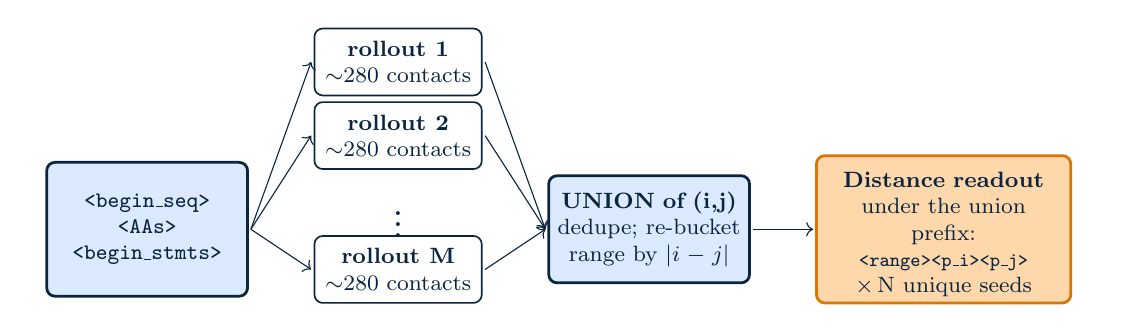
\begin{tikzpicture}[scale=0.85]
      % Base prompt box (left)
      \draw[draw=navy, line width=1pt, rounded corners=3pt, fill=lightnavy]
        (0, 0.5) rectangle (3, 2.5);
      \node[font=\footnotesize\ttfamily, text=navy, anchor=center,
            text width=2.8cm, align=center]
        at (1.5, 1.5) {<begin\_seq>\\<AAs>\\<begin\_stmts>};

      % Rollout boxes (middle-left)
      \foreach[count=\i from 0] \rr/\yy in {1/3.5, 2/2.4, M/0.4} {
        \draw[draw=navy, line width=0.6pt, rounded corners=3pt]
          (4.0, \yy) rectangle (6.5, \yy + 1.0);
        \node[font=\footnotesize, text=navy, anchor=center, align=center]
          at (5.25, \yy + 0.5)
          {\textbf{rollout \rr}\\$\sim$280 contacts};
        \draw[->, navy] (3.05, 1.5) -- (3.95, \yy + 0.5);
      }
      \node[font=\Large, text=navy] at (5.25, 1.7) {$\vdots$};

      % Union box
      \draw[draw=navy, line width=1pt, rounded corners=3pt, fill=lightnavy]
        (7.5, 0.7) rectangle (10.5, 2.3);
      \node[font=\footnotesize, text=navy, anchor=center, align=center,
            text width=2.8cm]
        at (9.0, 1.5) {\textbf{UNION of (i,j)}\\dedupe; re-bucket\\range by $|i-j|$};

      % Arrows from rollouts to union
      \foreach \yy in {0.9, 2.9, 4.0} {
        \draw[->, navy] (6.55, \yy) -- (7.45, 1.5);
      }

      % Readout box
      \draw[draw=orange, line width=1pt, rounded corners=3pt, fill=lightorange]
        (11.5, 0.4) rectangle (15.3, 2.6);
      \node[font=\footnotesize, text=navy, anchor=north, align=center,
            text width=3.6cm]
        at (13.4, 2.5)
        {\textbf{Distance readout}\\under the union\\prefix:\\
         \codeS{<range><p\_i><p\_j>}\\$\times$\,N unique seeds};
      \draw[->, navy] (10.55, 1.5) -- (11.45, 1.5);
    \end{tikzpicture}
  \end{center}
  \vspace{0.3em}
  Each rollout uses \codeS{logits\_processors=[ContactsOnlyLP(strategy="uniform")]},
  \codeS{T=0.7}, \codeS{top\_p=0.9}, \codeS{max\_tokens=900}.\\[0.2em]
  Union of $M=5$ rollouts gives $\sim$1500--10000 unique pairs per protein
  (deduped). The single readout under this rich prefix is the
  \codeS{sampled\_uniform\_M5\_union} distogram.
\end{frame}

% --- Slide 11: sampled alone results ---
\begin{frame}{Sampling alone vs pure iteration: complementary}
  \footnotesize
  \begin{center}
    \begin{tabular}{lrrr}
      \toprule
       & baseline & sampled\_uniform & iter\_R4\_grow \\
       & & M=5 union & \\
      \midrule
      mean LDDT     & 0.2496 & \textbf{0.3142} & \textbf{0.3511} \\
      $\Delta$\%    & --     & +25.9\%         & +40.7\%         \\
      chain wall (s)& 1387   & 2458            & 4373            \\
      \bottomrule
    \end{tabular}
  \end{center}
  \vspace{0.3em}
  Pure iteration wins overall, \emph{but} per-protein the two gain on
  DIFFERENT proteins:
  \vspace{0.2em}
  \begin{center}
    \begin{tabular}{lrrr}
      \toprule
      protein & baseline & iter\_R4\_grow & sampled M=5 union \\
      \midrule
      7y5j (L=102)  & 0.4485 & \textbf{0.5659} & 0.4521 \\
      7ykm (L=105)  & 0.3317 & \textbf{0.5178} & 0.3878 \\
      8eb9 (L=95)   & 0.1510 & 0.3071          & \textbf{0.3619 (+0.21!)} \\
      7zs2 (L=316)  & 0.2500 & 0.3619          & \textbf{0.3213} \\
      8cba (L=214)  & 0.2045 & 0.2735          & \textbf{0.2872} \\
      \bottomrule
    \end{tabular}
  \end{center}
  \vspace{0.2em}
  Iteration shines on the model's confident proteins; sampling unlocks
  the stuck ones. \textbf{Combine \textrightarrow{} next slide.}
\end{frame}

% --- Slide 12: combined algorithm ---
\begin{frame}{The combined algorithm}
  \begin{center}
    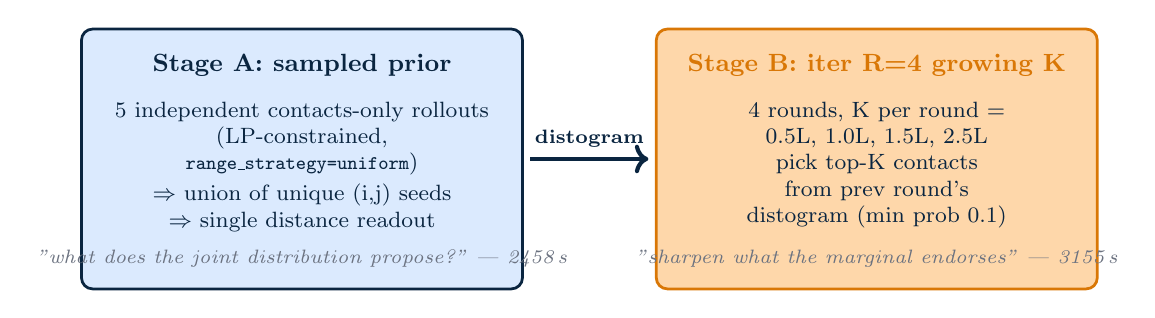
\begin{tikzpicture}[scale=1.0]
      % Stage A box
      \draw[draw=navy, line width=1pt, rounded corners=4pt, fill=lightnavy]
        (0, 0) rectangle (5.6, 3.3);
      \node[font=\small\bfseries, text=navy, anchor=north]
        at (2.8, 3.1) {Stage A: sampled prior};
      \node[font=\footnotesize, text=navy, anchor=north, text width=5.0cm,
            align=center]
        at (2.8, 2.5)
        {5 independent contacts-only rollouts\\
         (LP-constrained, \codeS{range\_strategy=uniform})\\[0.2em]
         $\Rightarrow$ union of unique (i,j) seeds\\
         $\Rightarrow$ single distance readout};
      \node[font=\scriptsize\itshape, text=grey, anchor=south]
        at (2.8, 0.15) {"what does the joint distribution propose?" — 2458\,s};

      % Arrow
      \draw[->, line width=1.5pt, navy] (5.7, 1.65) -- (7.2, 1.65)
        node[midway, above, font=\scriptsize\bfseries, text=navy] {distogram};

      % Stage B box
      \draw[draw=orange, line width=1pt, rounded corners=4pt, fill=lightorange]
        (7.3, 0) rectangle (12.9, 3.3);
      \node[font=\small\bfseries, text=orange, anchor=north]
        at (10.1, 3.1) {Stage B: iter R=4 growing K};
      \node[font=\footnotesize, text=navy, anchor=north, text width=5.0cm,
            align=center]
        at (10.1, 2.5)
        {4 rounds, K per round =\\0.5L, 1.0L, 1.5L, 2.5L\\
         pick top-K contacts from prev round's\\
         distogram (min prob 0.1)};
      \node[font=\scriptsize\itshape, text=grey, anchor=south]
        at (10.1, 0.15) {"sharpen what the marginal endorses" — 3155\,s};
    \end{tikzpicture}
  \end{center}
  \vspace{0.3em}
  \begin{center}
    \codeS{Final readout: <begin\_seq><AAs><begin\_stmts><range><p\_i><p\_j>...}\\
    {\footnotesize (R4 picks, $\sim 2.5L$ statements; long $>$ med $>$ short ordering)\\[0.2em]
     Standard E[d] = $\sum$ probs · midpoint. No sharpening.}
  \end{center}
  \vspace{0.6em}
  \begin{center}
    {\Large\bfseries\color{green}mean LDDT 0.3564 (+42.81\%)}\\
    {\small chain wall \textbf{5613\,s} (4.05$\times$ baseline; under 5$\times$).}
  \end{center}
\end{frame}

% --- Slide 13: per-protein result ---
\begin{frame}{Per-protein result of the combined algorithm}
  \begin{center}
    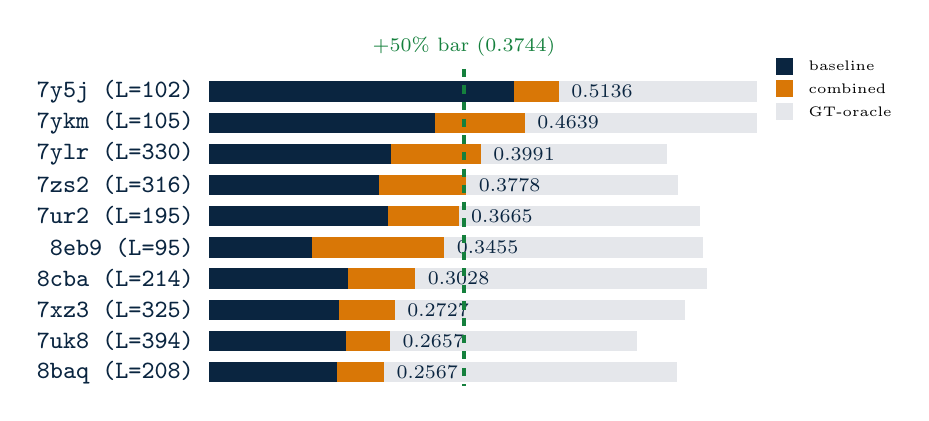
\begin{tikzpicture}[scale=0.72]
      \foreach[count=\i from 0] \name/\Len/\bv/\fv/\ov in {%
        7y5j/102/0.4485/0.5136/0.8044,
        7ykm/105/0.3317/0.4639/0.8052,
        7ylr/330/0.2673/0.3991/0.6734,
        7zs2/316/0.2500/0.3778/0.6895,
        7ur2/195/0.2633/0.3665/0.7219,
        8eb9/95/0.1510/0.3455/0.7254,
        8cba/214/0.2045/0.3028/0.7319,
        7xz3/325/0.1913/0.2727/0.6993,
        7uk8/394/0.2010/0.2657/0.6290,
        8baq/208/0.1872/0.2567/0.6870
        } {
        \pgfmathsetmacro\yp{-\i * 0.55}
        \node[anchor=east, text=navy, font=\small\ttfamily]
          at (-0.1, \yp) {\name\ (L=\Len)};
        \pgfmathsetmacro\wo{\ov * 12}
        \pgfmathsetmacro\wf{\fv * 12}
        \pgfmathsetmacro\wb{\bv * 12}
        \fill[lightgrey] (0, \yp - 0.18) rectangle ++(\wo, 0.36);
        \fill[orange] (0, \yp - 0.18) rectangle ++(\wf, 0.36);
        \fill[navy] (0, \yp - 0.18) rectangle ++(\wb, 0.36);
        \node[anchor=west, font=\scriptsize, text=navy]
          at (\wf + 0.05, \yp) {\fv};
      }
      \draw[green, line width=1.5pt, dashed]
        (4.493, 0.4) -- (4.493, -5.2);
      \node[anchor=south, font=\scriptsize, text=green]
        at (4.493, 0.45) {+50\% bar (0.3744)};
      \fill[navy] (10, 0.3) rectangle ++(0.3, 0.3);
      \node[right, font=\tiny] at (10.4, 0.45) {baseline};
      \fill[orange] (10, -0.1) rectangle ++(0.3, 0.3);
      \node[right, font=\tiny] at (10.4, 0.05) {combined};
      \fill[lightgrey] (10, -0.5) rectangle ++(0.3, 0.3);
      \node[right, font=\tiny] at (10.4, -0.35) {GT-oracle};
    \end{tikzpicture}
  \end{center}
  \vspace{-0.3em}
  {\footnotesize\color{navy}\textbf{5 / 10 proteins} pass the +50\% bar
    individually (up from 4 with iter\_R4\_grow alone).
    7ylr and 7zs2 cross the bar thanks to the sampled prior.\\
    Remaining 5 misses (8baq, 7uk8, 7xz3, 8cba, 8eb9) all gain
    +0.06 to +0.21 from baseline; their oracle ceilings are 0.62--0.73,
    so capacity exists but contacts still elude us.}
\end{frame}

% --- Slide 14: takeaways ---
\begin{frame}{Takeaways}
  \small
  \begin{itemize}
    \setlength\itemsep{0.3em}
    \item[\color{navy}\textbullet] \textbf{\codeS{<distance>} is not a boundary.}
      Training docs interleave contacts and distances; sampling without a
      grammar constraint stops after $\sim$10 contacts, leaving the seed set
      tiny.
    \item[\color{navy}\textbullet] \textbf{The model's range-token prior is
      pathologically biased.}
      $\sim$99\% medium-range when freely sampled. But all 3 ranges
      have similar entropy over the next position — \textbf{the
      conditional knowledge is there}.
    \item[\color{navy}\textbullet] \textbf{Force uniform range selection at
      sampling time.} Overwriting the 3 range-token logits to 0 in the LP
      gives 1/3 of each range; M=1 jumps from $-11\%$ to $+8.7\%$.
    \item[\color{navy}\textbullet] \textbf{Joint (sampling) and marginal
      (iteration) contact predictions are complementary.}
      Sampling unlocks the proteins iteration leaves stuck; iteration
      sharpens what sampling proposes. Combining them adds +0.005 over
      iteration alone.
    \item[\color{navy}\textbullet] \textbf{Still under the +50\% bar by 0.018.}
      The remaining gap is the model's honest contact-prediction quality on
      hard proteins, which neither sampling nor iteration can fully extract
      from this checkpoint at inference time.
  \end{itemize}
\end{frame}

% --- Slide 15: reproducer ---
\begin{frame}[fragile]{Reproducer}
  \scriptsize 10 proteins \textperiodcentered\ A100 40\,GB \textperiodcentered\ bf16
  \textperiodcentered\ vLLM 0.7.3 \textperiodcentered\
  total wall $\sim$5613\,s (4.05$\times$ baseline)
  \vspace{0.2em}
  \begin{lstlisting}[style=code,basicstyle=\ttfamily\scriptsize\color{navy}]
# 1. Sampled-uniform-M5 union prior (no naive baseline needed)
uv run python run_sampled_contacts.py --dtype bfloat16 --n-gpus 1 \
    --algorithm sampled_uniform_M5_union_T0.7 \
    --n-rollouts 5 --temperature 0.7 --top-p 0.9 --max-sample-tokens 900 \
    --range-strategy uniform --aggregation union
uv run python snapshot_distograms.py --to distogram_sampled_uniform_M5_union.npz

# 2. Iter R=4 grow on top
uv run python run_iterative.py --dtype bfloat16 --n-gpus 1 \
    --algorithm iter_R4_grow_on_sampled_uniform_M5 \
    --n-rounds 4 \
    --k-contacts-per-L-per-round 0.5 1.0 1.5 2.5 \
    --k-distances-per-L-per-round 0.0 0.0 0.0 0.0 \
    --min-contact-prob 0.1 \
    --prior-name distogram_sampled_uniform_M5_union.npz

# Result: mean LDDT 0.3564 (+42.81% over baseline 0.2496)
  \end{lstlisting}
  {\tiny\color{grey}\ttfamily Branch: exp/27-improved-inference-algorithm \textperiodcentered\
    Source: sampled\_contacts\_inference.py, iterative\_inference.py}
\end{frame}

\end{document}
